\section{问题一：斜坡上的覆盖宽度}

\subsection{问题分析与坐标关系}

平底条件下，覆盖条带关于测线对称；海底倾斜后，深水侧与浅水侧声束同坡面的交点不再对称，继续用平底宽度计算重叠率会混淆坡面长度与水平间距。本问的关键抽象是把测深过程投影到垂直测线的二维剖面，在同一水平坐标上描述水深、左右覆盖边界与相邻测线间距。

以海域中心为原点，令 $x>0$ 指向浅水上坡方向，竖直向下为水深正方向。由于海底为坡度 $\alpha$ 的直线，测线位置变化会直接改变换能器至海底的竖直距离。位置 $x$ 处的水深为

\begin{equation}
  D(x)=D_0-x\tan\alpha.
  \label{eq:q1_depth}
\end{equation}

式~\eqref{eq:q1_depth} 表明水深向浅水侧线性减小。模型只保留声束与坡面的水平交点坐标，使覆盖边界与后续测线间距具有相同量纲。

横向位置 $x$ 描述测线在海域中的水平位置，$D(x)$ 描述换能器至海底的竖直距离；两者均不同于声束传播长度。区分这三个量后，覆盖宽度可以直接作为布线约束，而无需在坡面长度和水平距离之间反复换算。

图~\ref{fig:q1_geometry} 给出统一的水平投影口径：$B_L$ 与 $B_R$ 分别表示测线两侧的水平半覆盖宽度，其和 $W$ 不是坡面长度，而是条带在水平面上的投影。

\begin{figure}[H]
  \centering
  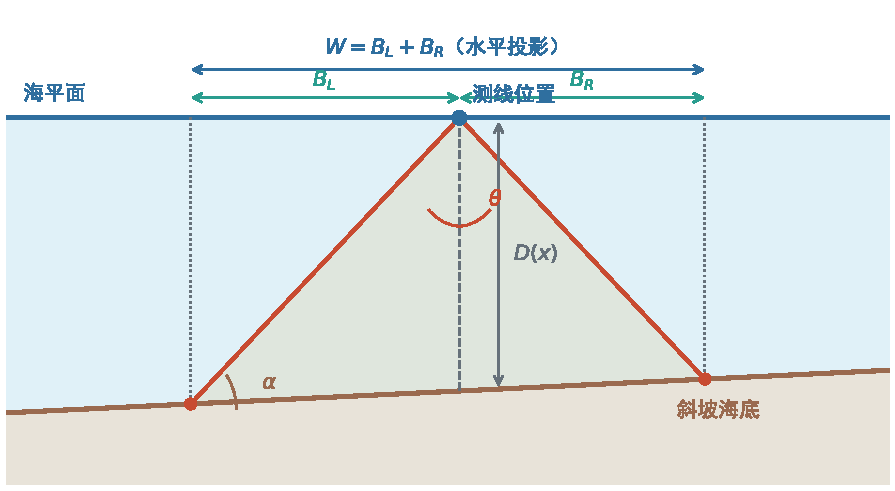
\includegraphics[width=0.82\textwidth]{../figures/q1/fig_q1_geometry.pdf}
  \caption{斜坡使左右半覆盖宽度不对称，而 $W=B_L+B_R$ 始终表示水平投影宽度}
  \label{fig:q1_geometry}
\end{figure}

\subsection{覆盖宽度模型}

声束边界同斜坡的交点决定条带两端。设半开角 $\phi=\theta/2$，由射线与斜坡直线的几何关系，左右半覆盖宽度的水平投影分别为

\begin{equation}
  B_L(x)=\frac{D(x)\sin\phi\cos\alpha}{\cos(\phi+\alpha)},\qquad
  B_R(x)=\frac{D(x)\sin\phi\cos\alpha}{\cos(\phi-\alpha)}.
  \label{eq:q1_half}
\end{equation}

分母中的 $\phi+\alpha$ 与 $\phi-\alpha$ 刻画斜坡对两侧声束的非对称作用。把两侧水平投影相加，可得条带覆盖宽度

\begin{equation}
  W(x)=B_L(x)+B_R(x)
      =D(x)\sin\phi\cos\alpha
      \left[\frac{1}{\cos(\phi+\alpha)}+\frac{1}{\cos(\phi-\alpha)}\right].
  \label{eq:q1_width}
\end{equation}

由于 $W(x)$ 与测线间距均为水平距离，二者可以直接用于覆盖判断。设相邻测线满足 $x_{i-1}<x_i$，水平间距为 $d_i=x_i-x_{i-1}$，则两条带在水平面上的代数重叠宽度为

\begin{equation}
  O_i=B_R(x_{i-1})+B_L(x_i)-d_i.
  \label{eq:q1_overlap_width}
\end{equation}

$O_i>0$ 表示重叠，$O_i<0$ 表示两条覆盖边界之间存在缺口。为与当前测线的覆盖能力比较，定义

\begin{equation}
  \eta_i=\frac{O_i}{W(x_i)}\times100\%.
  \label{eq:q1_overlap}
\end{equation}

该定义保留负值，因此同一指标既能表示冗余程度，也能直接识别漏测。

式~\eqref{eq:q1_overlap_width} 将前一条测线向浅水侧的覆盖范围与后一条测线向深水侧的覆盖范围相加，再扣除测线间距；以当前条带宽度归一化后，不同水深位置的重叠程度可以比较。

归一化分母取当前测线的条带宽度，使题面给定的各位置计算采用同一口径。代数重叠量保留负号：正值对应重复测量，负值的绝对值直接给出两条带之间的水平缺口，从而把冗余与漏测纳入同一判据。

\subsection{计算结果与规律}

取 $\theta=120^\circ$、$\alpha=1.5^\circ$、$D_0=70\text{ m}$，对题面给定的 9 个位置计算，结果见表~\ref{tab:q1}。

\begin{table}[H]
  \centering
  \caption{问题一各测线位置的水深、水平覆盖宽度与相邻重叠率}
  \label{tab:q1}
  \resizebox{\textwidth}{!}{%
    \begin{tabular}{lrrrrrrrrr}
      \toprule
      测线距中心点距离 / m & $-800$ & $-600$ & $-400$ & $-200$ & $0$ & $200$ & $400$ & $600$ & $800$ \\
      \midrule
      海水深度 / m & 90.95 & 85.71 & 80.47 & 75.24 & 70.00 & 64.76 & 59.53 & 54.29 & 49.05 \\
      覆盖宽度 / m & 315.71 & 297.53 & 279.35 & 261.17 & 242.99 & 224.81 & 206.63 & 188.45 & 170.27 \\
      重叠率 / \% & -- & 35.70 & 31.51 & 26.74 & 21.26 & 14.89 & 7.41 & $-1.53$ & $-12.36$ \\
      \bottomrule
    \end{tabular}%
  }
\end{table}

从深水侧向浅水侧移动时，水深由 $90.95\text{ m}$ 降至 $49.05\text{ m}$，覆盖宽度相应由 $315.71\text{ m}$ 单调降至 $170.27\text{ m}$。当相邻测线仍保持 $200\text{ m}$ 间距时，覆盖能力的下降不断消耗重叠余量：重叠率从 $35.70\%$ 降至 $-12.36\%$，并在 $x=600\text{ m}$ 处转为负值。这意味着固定间距同时造成深水侧冗余和浅水侧漏测，测线间距应随局部水深减小而收缩。图~\ref{fig:q1_result} 将这一因果链集中展示。

重叠率比覆盖宽度变化更敏感，因为它同时取决于前后条带边界与固定间距。当覆盖宽度接近 $200\text{ m}$ 时，水深继续下降会使正重叠迅速转为漏测，因此布线必须逐对检查相邻条带。

表格负责给出各位置的精确数值，图~\ref{fig:q1_result} 用于观察水深、覆盖宽度和重叠率的同步变化。浅水端的负重叠表明，按中心水深或平均宽度设置固定间距不能保证全域连续覆盖；后续布线应根据局部水深逐步收缩间距。

\begin{figure}[H]
  \centering
  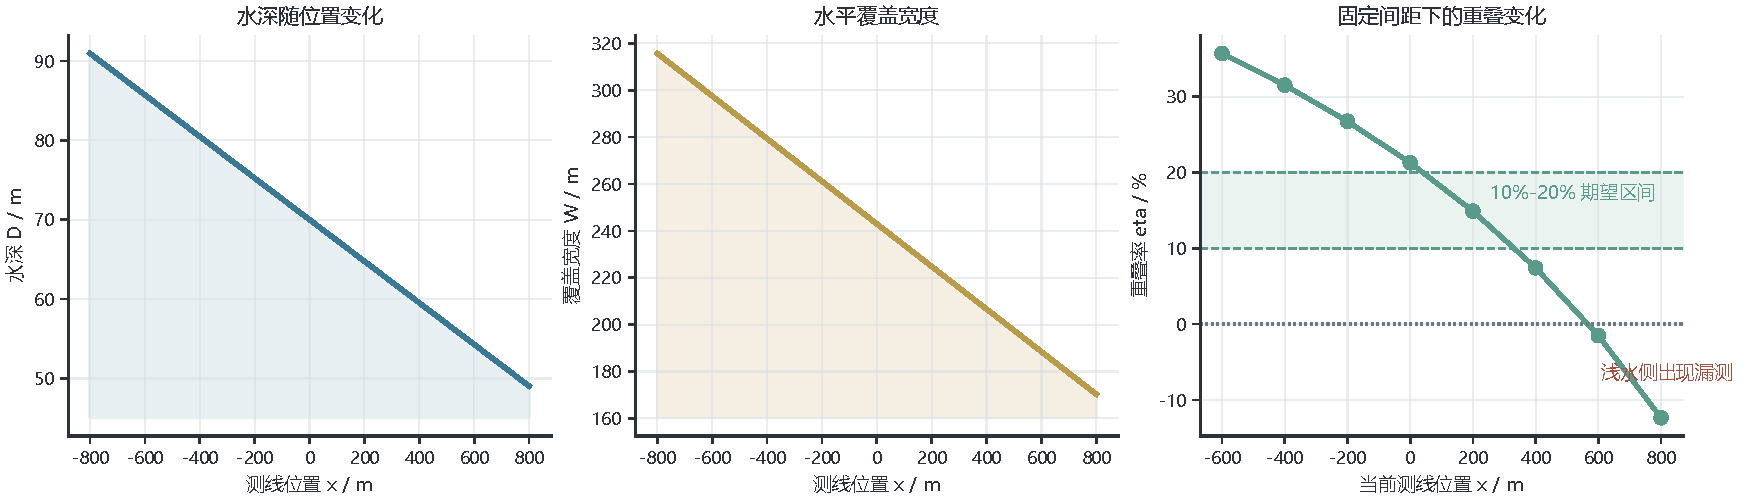
\includegraphics[width=1.0\textwidth]{../figures/q1/fig_q1_result.pdf}
  \caption{水深减小使水平覆盖宽度收缩，并推动固定间距下的重叠率由正转负}
  \label{fig:q1_result}
\end{figure}

\subsection{极限检验与敏感性分析}

当 $\alpha=0$ 时，式~\eqref{eq:q1_half} 退化为 $B_L=B_R=D\tan\phi$，进而有 $W=2D\tan(\theta/2)$、$\eta=1-d/W$，与题面平底公式一致。这一极限检验说明，水平投影口径在斜坡消失时能够无缝回到已知关系。

为比较两个几何参数的影响，在 $x=0$、$D_0=70\text{ m}$ 处分别扰动坡度与开角，结果见表~\ref{tab:sens}。

\begin{table}[H]
  \centering
  \caption{中心位置覆盖宽度对坡度和开角的单因素敏感性}
  \label{tab:sens}
  \begin{tabular}{lcccccc}
    \toprule
    $\alpha$ / $^\circ$（$\theta=120^\circ$） & 0.0 & 0.5 & 1.0 & 1.5 & 2.0 & 3.0 \\
    $W$ / m & 242.49 & 242.54 & 242.71 & 242.99 & 243.38 & 244.50 \\
    \midrule
    $\theta$ / $^\circ$（$\alpha=1.5^\circ$） & 100 & 110 & 120 & 130 & 140 & -- \\
    $W$ / m & 167.01 & 200.22 & 242.99 & 301.18 & 386.65 & -- \\
    \bottomrule
  \end{tabular}
\end{table}

坡度从 $0.0^\circ$ 增至 $3.0^\circ$ 时，覆盖宽度仅增加 $2.01\text{ m}$；开角从 $100^\circ$ 增至 $140^\circ$ 时，覆盖宽度则由 $167.01\text{ m}$ 增至 $386.65\text{ m}$。因此在本题小坡度范围内，开角决定基本覆盖尺度，水深变化决定沿程收缩趋势，坡度主要造成两侧覆盖不对称。

坡度对总宽度的影响较小，但仍会改变 $B_L$ 与 $B_R$ 的分配；后续模型因此保留等效坡度和左右半宽。

上述敏感性分析只比较单因素变化，不改变题面参数与主结果。它说明开角决定基本覆盖尺度，水深决定沿程收缩趋势，而坡度通过左右半宽的不对称影响相邻条带衔接。

本问解决了固定横断面内“覆盖多宽”的问题，但实际测线航向会同时改变船位水深和横断面坡度。下一问保留上述水平投影模型，仅把恒定坡度替换为航向坐标系中的等效坡度，由此将二维覆盖关系推广到三维海域。
